\documentclass[titlepage,12pt,a4paper]{article}

\usepackage[left=2cm,top=3cm,right=2cm,bottom=3cm,bindingoffset=0.5cm]{geometry}
\usepackage{amsmath}
\usepackage{amssymb}
\usepackage{enumitem}
\usepackage{commath}
\usepackage{mathtools}
\usepackage{graphicx}
\usepackage{dirtytalk}
\usepackage{csquotes}
\usepackage{hyperref}
\usepackage{tabto}
\usepackage{gensymb}
\usepackage{graphicx}
\usepackage{listings}
\usepackage{sidecap}
\usepackage{wrapfig}
\usepackage{parskip}

\usepackage{fancyhdr}
\usepackage{color}
\definecolor{dkgreen}{rgb}{0,0.6,0}
\definecolor{gray}{rgb}{0.5,0.5,0.5}
\definecolor{mauve}{rgb}{0.58,0,0.82}

\lstset{frame=tb,
  language=C++,
  aboveskip=3mm,
  belowskip=3mm,
  showstringspaces=false,
  columns=flexible,
  basicstyle={\small\ttfamily},
  numbers=left,
  numberstyle=\footnotesize,
  stepnumber=1,
  numbersep=5pt,
  keywordstyle=\color{blue},
  commentstyle=\color{dkgreen},
  stringstyle=\color{mauve},
  breaklines=true,
  breakatwhitespace=true,
  tabsize=3
}


\pagestyle{fancy}\lhead{A} \rhead{C}
\chead{{\large{\bf B}}}
\lfoot{}
\rfoot{\bf \thepage}
\cfoot{}

\setlength{\headheight}{15.2pt}
\pagestyle{fancy}
\fancyhf{}
\lhead{ \fancyplain{}{COMP3431: Robotic Software Architecture} }
\rfoot{ \fancyplain{}{\thepage} }


\begin{document}
\begin{titlepage}
    \begin{center}
        \vspace*{3cm}
        
        \Huge
        \textbf{COMP3431\\}
        \title{}
        \vspace{0.5cm}
        \Huge
        \textbf{Robotic Software Architecture}
        
        \vspace{0.54cm}
        
        \Large
        Assignment 1: Report
        
        \vspace{5cm}

	\normalsize
	Christopher Manouvrier\\
	Aaron Ramshaw\\
	Simon Robilliard\\
	Oliver Tan\\
	Aneita Yang
        
	\vfill
        
        \Large
        September 11, 2015
        
    \end{center}
\end{titlepage}

\pagebreak
\tableofcontents

\pagebreak
\section{Architecture}
The objective of this assignment is to autonomously navigate an unknown maze and visit beacons in a specified order. To achieve this goal, the assignment is broken down into three main modules - exploration, beacon recognition and localisation and waypoint traversal. We also have two modules which aid us in providing or processing data - the movement and odometry modules, and a shared library handling typical robot movement and occupancy grid processing.

\subsection{Main Modules}
In exploration, the TurtleBot's task is to map out an unknown maze while avoiding obstacles (walls and beacons). The TurtleBot achieves this by performing a frontier-based search on the data gathered from its laser scan. 

In the beacon module, beacons are pinpointed using the Bot's camera. This information is then combined with the data from the laser scan to determine the position of the beacons. This module is also responsible for keeping track of when the TurtleBot has recognised all four required beacons. 

Waypoint traversal guides the TurtleBot from beacon to beacon. The path the TurtleBot takes is determined by an A* search, using Euclidean distance to the goal as the heuristic. 

There are two phases in this assignment: the exploring phase, and the waypoint traversal phase. The exploration module is run in conjunction with the beacon module to simultaneously map the maze and locate beacons. Once the beacon module has detected the four required beacons, a message is sent signalling for waypoint traversal to begin. 

\subsection{Helper Modules}
\subsubsection{Movement Module}
The movement module processes all movement actions generated by exploration or waypoint traversal. 

If the movement is deemed to be unsafe (as it hits walls), the movement module will prevent all exploration or waypoint actions, and aims to move the bot in a position such that it is at least 30cm from any wall. Otherwise, it forwards data onto \verb|/cmd_vel_mux/navi|. 

For ease of figuring out when it will crash into a wall, we limit all movement to be either in the x direction, or the angular z direction.

The accepted value from the wall to the robot is 30cm.

\subsubsection{Odometry Module}
Our custom odometry module waits for a transform from \verb|/map| to \verb|base_link|, such that it always publishes a valid odometry reading in map coordinates. This is published on \verb|ass1/odom|, and is subscribed to instead of \verb|/odom|. This allows us to reference all objects relative to the same origin.

\subsection{Mapping}
For mapping, FastSLAM is used for its speed and accuracy to generate the map. Although HectorSLAM produces a higher resolution map (0.01), it does take longer for A* to work on. FastSLAM's 0.05 resolution is sufficient for our purposes.

\subsection{Helper Libraries}
We have chosen to use shared libraries instead of additional ROS nodes, to lower communication and prevent more handling of callbacks (concurrency is hard enough!). These libraries are used by all the main modules to aid with processing common routines.

\subsubsection{astar.h}
\verb|astar.h| is a generic A* library that allows us to perform A* search on grid-based maps. It works by passing in a State class, which has their own definitions of "goal" state, the heuristic and methods to explore the maze. State examples are also in \verb|astar.h|.

\subsubsection{bot.h}
\verb|bot.h| contains typical routines that help with localising the bot have such as generating movement directions, and figuring out where the bot is. It requires setting up an extra callback from our own odometry module.

\subsubsection{maze.h}
\verb|maze.h| contains information on the occupancy grid, and contains routines that allow us to process data regarding the maze as well as wall fattening. It requires setting up an extra callback from the \verb|/map| channel.

\pagebreak
\section{Operation}
\subsection{Exploration}
Before it can visit beacons in a specified order, the TurtleBot must first explore the maze. To begin the exploration phase, the TurtleBot waits for an OccupancyGrid message and an Odom message to ensure the robot's start-up has been successful. 

Exploration of the maze can be completed using a simple wall-follower, or by performing a search algorithm. A wall-follower, although guaranteed to map out the entire maze correctly, has limitations in its speed. It often spends more time than is necessary to finish mapping a location, following any walls it comes across, regardless of any existing knowledge about the area.

Thus, to speed up the exploration of the unknown maze, a frontier-based search is performed on any existing data we have of the maze. This data is delivered to us in the form of an OccupancyGrid message, which publishes an array of integers from -1 to 100 representing knowledge of the maze. The search looks for the closest frontier of unknown points (-1) or uncertain points (20-80\% chance) in the OccupancyGrid and the TurtleBot is instructed to explore this closest frontier. By moving to this frontier, the TurtleBot is able to expand its map until the entire maze has been explored. 

To calculate the movements required by the TurtleBot to reach its goal, we consider the location of the robot and its goal in global coordinates. Letting $\theta$ be the angle of the target from the TurtleBot and $d$ be the distance of the target from the TurtleBot:

\begin{align*}
	d			&=	\sqrt{(x_{BOT} - x_{TARGET})^2 + (y_{BOT} - y_{TARGET})^2} \\
	\theta		&=	\tan^{-1}{(\frac{y_{TARGET} - y_{BOT}}{x_{TARGET} - x_{BOT}})} 
\end{align*}

Then, if $\theta_m$ is the angle of the target from the origin of the map:
\begin{align*}
		\theta_m 	&=	\theta - \text{bot}_{yaw} 
\end{align*}

$d$ and $\theta_m$ are written to a Twist message which is published.

\begin{figure}[h]
	\begin{center}
	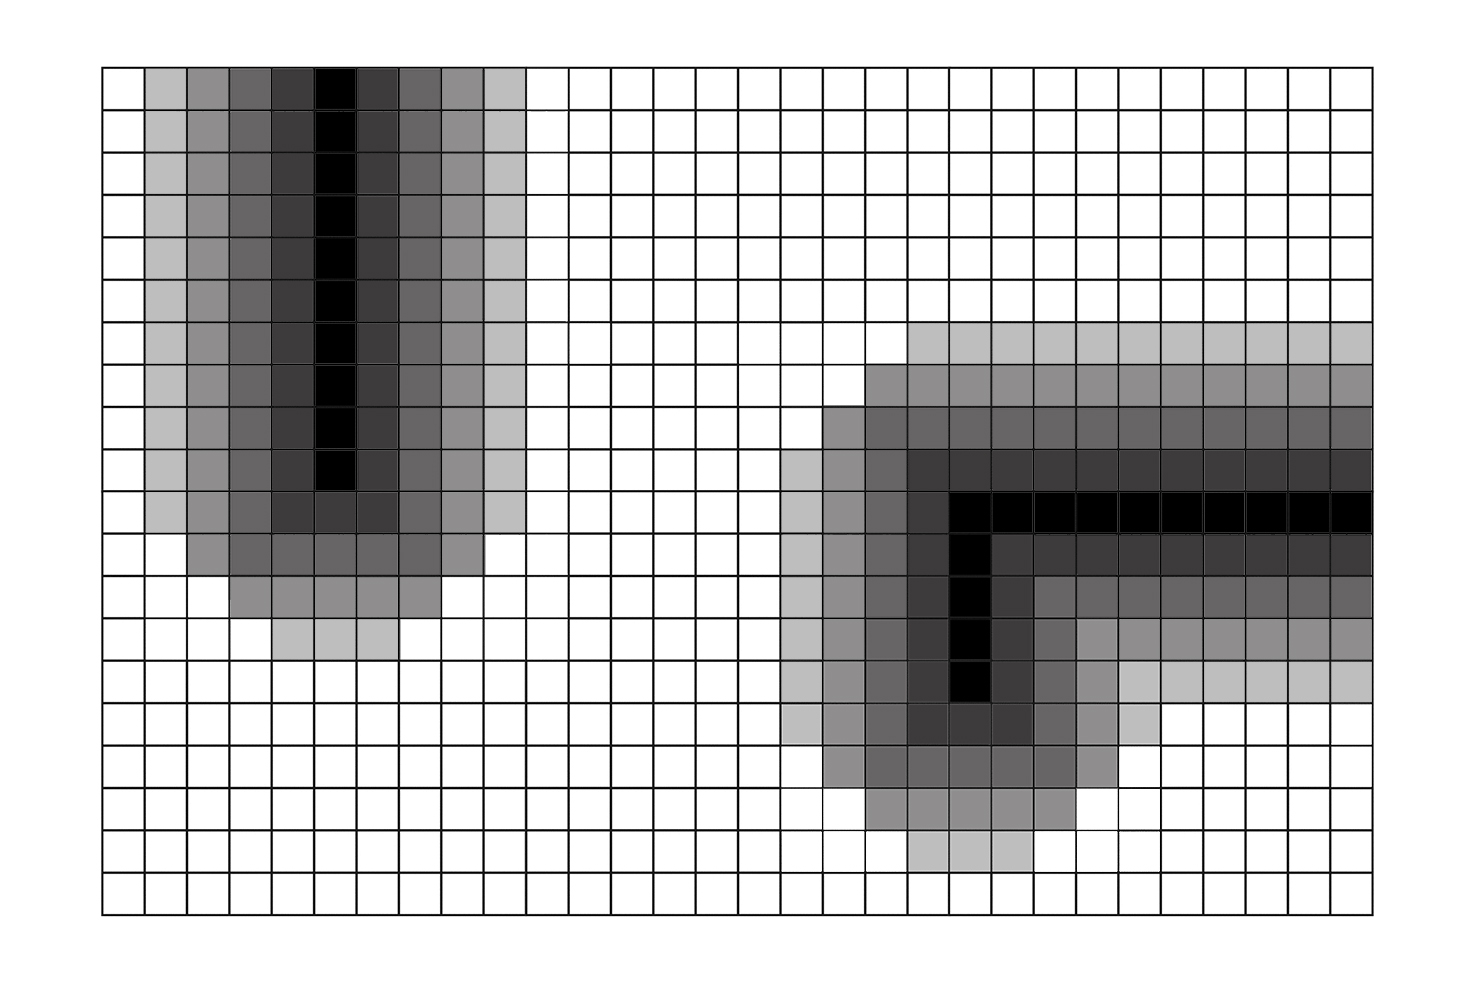
\includegraphics[scale=0.25]{wallfatten.jpg}
	\caption{Example of wall fattening by 4 cells, where black is the original wall}
	\end{center}
\end{figure}

As another safety measure, any cells in the OccupancyGrid with an occupancy probability greater than 95 are treated as having 100\% occupancy and are ``fattened" by 20cm. Given that the TurtleBot's radius is 15cm, this gives the robot a 5cm leeway from the walls, and a 60cm-wide pathway to travel along. To ``fatten" the walls, we occupy the rings of cells surrounding every wall in the current OccupancyGrid (Figure 1). Fattening the walls also blocks any gaps between the walls that the robot may have originally seen through. 

A frontier-based search is advantageous in that the robot can explore areas with an arbitrary number of obstacles (walls and beacons) and loops that may confuse a wall-follower no longer become an issue. 

As the OccupancyGrid is continually being updated, the frontier-based search also increases the speed of the search by eliminating the need for the TurtleBot to travel down dead-ends. Whereas a wall-follower would lead the Bot into the dead-end, the frontier-based search will not. 

However, this may mean beacons could be missed if the laser scan can infer a corner, and hence skips it. But our movement seemed to be in such a way that it peers through each corner, so we leave it as is.

\begin{figure}[h]
	\centering
	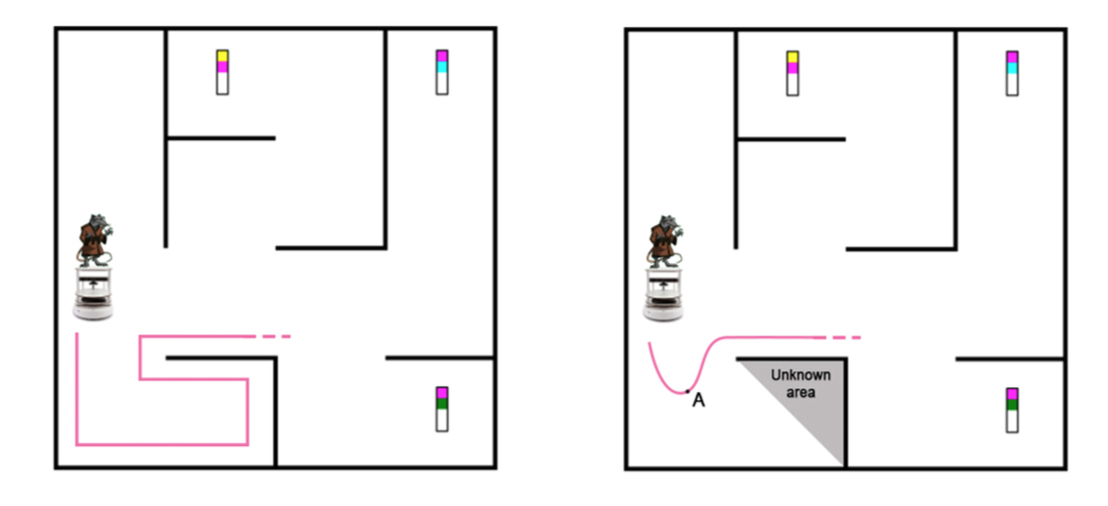
\includegraphics[scale=0.7]{paths.png}
	\caption{\textbf{Left:} Example of wall following exploration in a dead-end. \textbf{Right:} Example of frontier-based search in a dead-end.}
\end{figure}

\pagebreak
\begin{figure}[h]
	\centering
	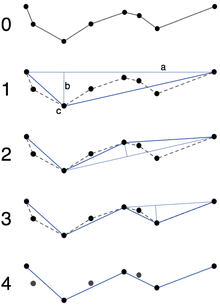
\includegraphics[scale=0.5]{rdp.png}
	\caption{RDP}
\end{figure}
	
As the frontier-based search is performed on a map with a resolution of 0.05, the resulting path can often be jagged and over-complicated. In order to smooth-out our path, the Ramer-Douglas-Peucker algorithm is used to reduce the number of intermediary points in the path (see Appendix). RDP works by recursively dividing a given path, finding an intermediary point that is the furthest from the line segment drawn from the start to the end of a path. If the distance of this furthest point is within the given threshold, the point can be discarded, thus, cutting down the number of intermediary points the TurtleBot must visit. A threshold of 0.055 is used in our RDP path simplification, meaning that points that lie within 5.5cm can be overlooked.

As movement can be interrupted due to proximity to walls, when the movement module interrupts to perform unsticking actions, an A* is used to recalculate the path to the destination - here we use the Waypoint A* state as it is the same idea. However, as the target may be a wall, we recalculate to be up to 50cm back from where the original target was. This action further guarentees that the Kinect can see all beacons, even if a corner is missed due to the recalculation, and the unsticking action finding a wall.

\pagebreak
\subsection{Beacon Recognition and Localisation}

\subsubsection{Detection}
During the TurtleBot's first exploration of the maze, the camera is used to identify and position beacons. The beacon finder node subscribes to RGB images from the Kinect camera and processes them using OpenCV. The following criteria is used to detect the beacons:

    \begin{enumerate}
        \item Colour range filtering to see only and distinguish pink, blue, green and yellow colours of the beacons.
        \item Simple blob detection to find beacon shaped objects:
        \begin{enumerate}
            \item Area greater than 200 pixels.
            \item Inertia greater than 0.65.
            \item Convexity greater than 0.5.
        \end{enumerate}
    \end{enumerate}

The blob detector produces key points in the form of coordinates on the 640 * 480 RGB image, in the center of the beacon colour block. We conclude that a beacon has been successfully detected if there are two ``blobs" in the same image frame within a 20 pixel offset from each other in the horizontal x axis. This threshold of 20 pixels is used to account for any motion blur. The beacon's top colour is determined by comparing the two keypoints' y values.

We also use the laser scan data to find the location of the beacon relative to the bot by reading the laser data at the angle corresponding to the angle on the RGB image. This information is then used in conjunction with the odom to give the location of the beacon with respect to the global map. 

\subsubsection{Localisation}
Pinpointing the locations of detected beacons is essential in order for the TurtleBot to complete waypoint traversal. Each beacon's position is determined by first considering the TurtleBot's position and orientation in the maze (i.e. relative to the origin of the map), and looking at the ranges array from the laser scan. 

To determine the rotation of the beacon from the origin of the map, we consider the pixel in the image at which the beacon was detected, relative to the centre pixel of the image. It is known that the camera has a 58\degree field-of-view and, thus, we are able to use these pixel values to calculate the beacon's rotation from the origin. 

\begin{figure}[h]
	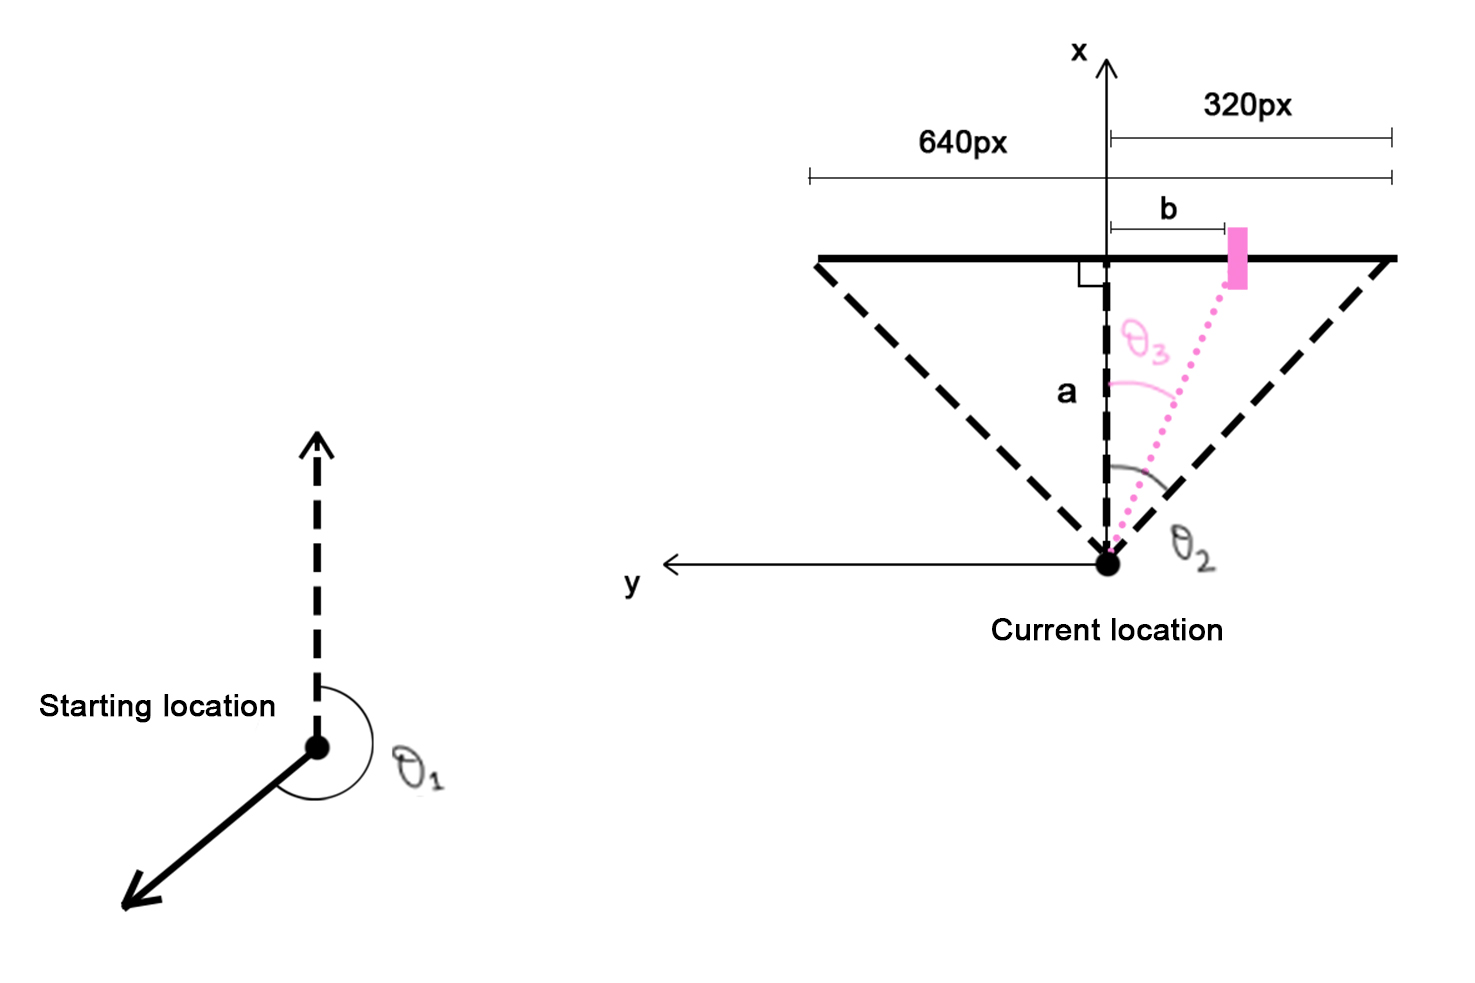
\includegraphics[scale=0.3]{beacon.jpg}
	\caption{Beacon localisation}
\end{figure}

\begin{align*}
	\theta_1   &=  \text{TurtleBot's current yaw, relative to start} \\
	\theta_2   &=  29\degree \\
	\\
	a 	        &=  \frac{320}{\tan{29\degree}} \\ 
	b 	        &=  \text{position of beacon given as an offset from centre of image} \\
			&=  \text{vertical pixel in image at which beacon was detected} - 320\text{px} \\
	\\
	\theta_3   &= \tan^{-1}{(\frac{b}{a})} \\
		        &= \tan^{-1}{(\frac{b \cdot \tan{29\degree}}{320})} 
\end{align*}

Therefore, the beacon's yaw from the TurtleBot is $\theta_3$ and the beacon's yaw from the origin of the map is $\theta_1 + \theta_3$. Note that in the above example, $\theta_3$ is negative as tan is negative in the fourth quadrant.

To determine the beacon's x and y coordinates in the map, we consider the TurtleBot's position, the beacon's angle from the TurtleBot ($\theta_3$), and the array of ranges gathered from the laser scan. 

\begin{align*}
	\text{beacon.x}		&=		\text{bot.x} + d \cdot \cos{(\theta_1 + \theta_3)} \\
	\text{beacon.y} 		&= 		\text{bot.y} + d \cdot \sin{(\theta_1 + \theta_3)} 
\end{align*}
Letting $\theta_{BL}$ be the angle of the beacon with respect to the laser: 
\begin{align*}
		\theta_{BL}	&= 		\text{beacon.yaw} - \text{laser.angle\_min} \\
   \text{beacon\_index}	&=		\frac{\theta_{BL}}{\text{laser.angle\_increment}} \\
   					 \\
				d 	&=		\text{beacon's distance from TurtleBot} \\
					&=		\text{laser.ranges [ beacon\_index ]} 
\end{align*}

Using the ranges array gathered from the laser scan eliminates the need for the TurtleBot to be next to the beacon to pinpoint its location. Rather, once a beacon is within the camera's view, it's position can be determined, speeding up the process of beacon localisation. In turn, the TurtleBot's initial exploration is also sped up.

\pagebreak
\subsection{Planner}

The planner requirement in the assignment specification is merged into the beacon recognition module.

A vector of four Beacon objects is created when the beacon recognition module first begins, where the first index holds the first beacon to visit, the second index holds the second beacon to visit, and so on. Beacon objects store the top and bottom colour of the beacon as strings, x and y coordinates, and a boolean value as to whether the beacon has been found within the maze. 

As beacons are detected during the exploration phase, their positions are stored in the vector. Once the four beacons have been found, their coordinates are moved from the vector to a FoundBeacons message which is published, signalling to the Exploration module to shutdown and the Waypoint Traversal module to begin. Image data is also terminated on the beacon recognition module, as we have all positions, so data is no longer required.

This essentially allows our TurtleBot to stop exploring the maze once all four beacons have been detected, regardless of whether the robot has finished exploring the entire maze.

\textbf{Beacon Class}
\begin{lstlisting}
	class Beacon {
	public:
    		double x, y;
    		bool known_location;
    		string top, bottom;

    		Beacon(string top, string bottom) :
        			x(0), y(0),
        			known_location(false),
        			top(top), bottom(bottom) {}

    		bool found() {
        			return known_location;
    		}
	};
	
\end{lstlisting}

\textbf{\\FoundBeacons Message}
\begin{lstlisting}[language=C++]
	int32 n
	geometry_msgs/Point[] positions
\end{lstlisting}

\pagebreak
\subsection{Waypoint Traversal}

Once the FoundBeacons message is published, the TurtleBot will switch from its exploration phase to waypoint traversal.

To speed up the traversal between beacons, an A* search is performed on the available data - namely, the OccupancyGrid and the FoundBeacons message which contains the positions of the beacons. The search considers all the neighbouring cells of the current location and the neighbouring cell's Euclidean distance from the goal (the beacon) to find the shortest path. 

A search is first performed to find a path between the TurtleBot's current location and the first beacon. We consider a TurtleBot to have reached the goal beacon if it is within a 30cm radius of the beacon - to counteract the wall set by the occupancy grid fattener. That is, if: 

\begin{align*}
	\sqrt{(x_{BOT} - x_{BEACON})^2 + (y_{BOT} - y_{BEACON})^2} \leq 0.3m 
\end{align*}

Once the TurtleBot reaches the beacon, another search is performed to find the path to the next beacon.

\begin{figure}[h]
  	\begin{center}
	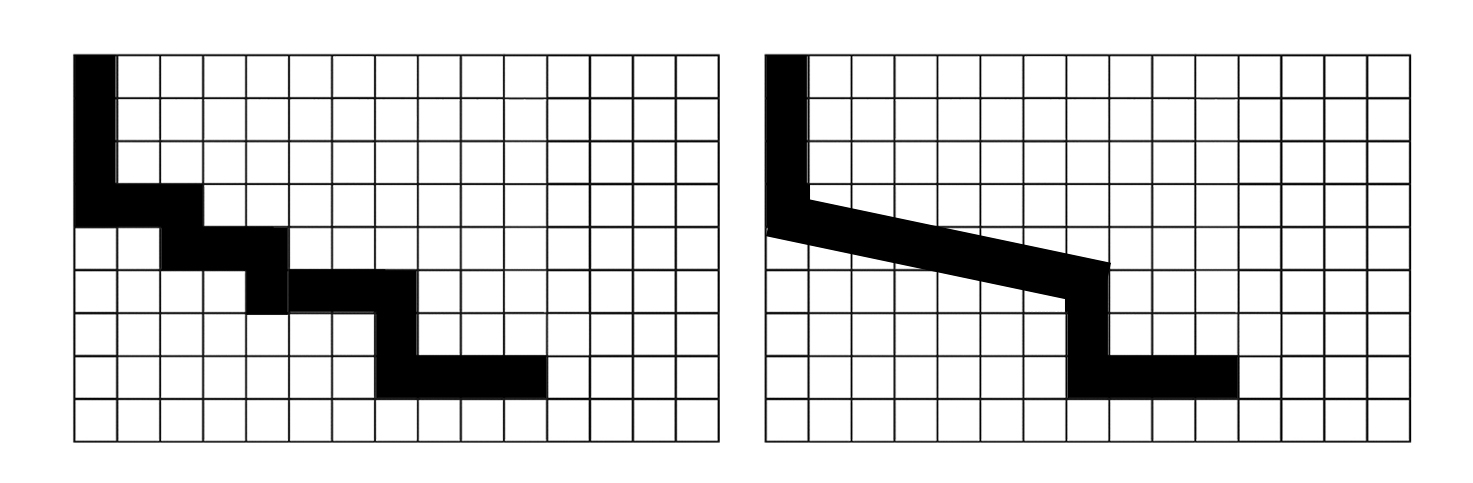
\includegraphics[scale=0.27]{rdpExample.jpg}
	\caption{\textbf{Left:} Original A* path. \textbf{Right:} RDP simplified path}
	\end{center}
\end{figure}

As the search is performed on a high-resolution map (0.05m/cell), the resulting path can be jagged and over-complicated. Like in the exploration phase, a Ramer-Douglas-Peucker path simplification is performed on each path that is returned from the A*, cutting down on the number of intermediary points the TurtleBot must visit.

To move from beacon to beacon, the same movement logic from the exploration module is used and the laser's array of ranges is used to detect any potential collisions. However, if an unstuck action is performed, an A* to the same goal is remade.

\pagebreak
\section{Results}
During exploration, the robot managed to look at every corner as it goes through the maze with the laser and our frontier exploration into an unknown or uncertain cell. There were fears that as the frontier search does not do a second round, and the laser's higher angle compared to the Kinect, we would not be able to see all four beacons. However, all four required beacons were recognised before the 8 minute mark.

However, during waypoint traversal, we had some mixed results:

\begin{itemize}
	\item The first beacon was found and reached successfully.
	\item The second beacon was around a corner, which the Kinect just managed to see through as the bot turned to look in that corner, and the laser successfully mapping it. With our beacon localisation strategy of bringing the beacon 30cm forward, and the tight angle, the beacon was reported to be at an incorrect location, a cell off, as it was reported to be on the other side of the wall. However, waypoint successfully navigated to that location.
	\item The third beacon was found and reached - however, due to some inaccuracies, it was placed in the wall. The robot kept trying to get into the wall - but our movement prevented this from happening. This meant our waypoint "targeting" was uncalibrated - which was true, as we increased the wall fattening to 5 units at the last minute. 
	\item Nudging the bot against the wall to mark the bot as seen the third beacon, the bot successfully visited the last beacon, albeit overtime at about 16 minutes and 30 seconds from start.
\end{itemize}

Movement by the bot was ineffective when trying to turn any corner. As we only allow forward xor angular movements, this made it turn through corners too straight - thus increasing likelihood of the movement module detecting it was too close to the wall, requiring the bot to reverse and try turn the corner again - but then being too close to the wall. We thought having more circular walls would prevent this, but the effect was limited. The net result was in a longer period of time navigating the maze. However, with RDP, straight lines were efficient.

Overall, a success with a few hiccups. All components integrated together - just a few values that required more fine tuning.

\pagebreak
\section{Future Improvements}

\subsection*{Movement}
One of the biggest optimisations is time - and with our movement strategy, it was slow around the corner. We believe that with our strategy of only turning xor walking straight impacted us - and moving forwards whilst turning in an arc may have prevented what we have observed. 

As mentioned earlier, fattening the walls would have been another strategy, as the A* would return a path that does not hit the walls. However, make it too fat, and the A* may not be able to "cross" the wall.

\subsection*{Potentially missing corners on Exploration} 
We believe that the bot may miss corners. To prevent this, we could have set up a secondary structure to keep track of where the bot has been before in terms of metre by metre cells, and reconfigure the A* to search this cell if necessary. 

\subsection*{Beacon Localisation}
As shown in results, beacons could be recognised but localised incorrectly.

One strategy would have been to instead use the Kinect DepthCloud, which provided a more accurate distance measurement. 

Another would have been to store a position of where we think the beacons are, and take the average after applying a Kalman filter to filter outliers. However, this might have been missed during exploration as the laser scanner marks the cell as explored and moves along. To prevent this, the exploration would have to take in the exploration improvement mentioned above.

Another strategy would have been to only mark beacons as explored once the Kinect sees the colour beacon again, and marks the beacon as close enough. In other words, we should have followed the spec, and had a planner module keep track of beacons as they are found and explored. This would have also potentially saved time during exploration - in which beacons found already in order could be ignored during waypoint traversal!

\subsection*{More tests - on powered up TurtleBots!}
TurtleBots were always low on battery, with all 6 groups using all 5 bots. This made it hard to test, as it was always running out of charge. More experimentation and refinement could have been made in the allocated timeframe if this was fixed. That said, we could have started earlier...

\pagebreak
\section{Appendix}

\subsection{Ramer-Douglas-Peucker Path Simplification}
\begin{lstlisting}[language=C++]
	static vector<pair<double,double>> rdp_simplify(vector<pair<double, double>> in, double threshold) {
        vector<pair<double, double>> out;
        if (in.size() > 2) {
            // Find the vertex furthest from the line defined by the
            // start and the end of the path
            double max_dist = 0;
            size_t max_dist_i = 0;      

            pair<pair<double,double>,pair<double,double>> line = make_pair(in.front(), in.back());
    
            for (size_t i = 0; i < in.size(); i++) {
            	// Calculate the distance from the line to the point
                double dist = distance_line_point(line, in[i]);
                if (dist > max_dist) {
                    max_dist = dist;
                    max_dist_i = i;
                }
            }

            // If furthest vertex is greater than our threshold, we
            // partition and recursively call on left and right
            if (max_dist > threshold) {
                // Partition 'in' into left and right subvectors,
                // and optimize them
                vector<pair<double, double>> left;
                vector<pair<double, double>> right;
                
                for (size_t i = 0; i < max_dist_i + 1; i++) {
                    left.push_back(in[i]);
                }
                for (size_t i = max_dist_i; i < in.size(); i++) { 
                    right.push_back(in[i]);
                }
	
                vector<pair<double, double>> leftSimplified = rdp_simplify(left, threshold);
                vector<pair<double, double>> rightSimplified = rdp_simplify(right, threshold);

                // Combine optimised paths
                out.clear();
                for (size_t i = 0; i < leftSimplified.size(); i++) {
                    out.push_back(leftSimplified[i]);
                }
                for (size_t i = 1; i < rightSimplified.size(); i++) {
                    out.push_back(rightSimplified[i]);
                }
            } else  {
                out.push_back(line.first);
                out.push_back(line.second);
            }
            // Return optimised path
            return out;
        } else {
        	    // Return original path
            return in;
        }
    }    
\end{lstlisting}


\end{document}
